\documentclass[bibliography=totoc]{scrartcl}
\usepackage[ngerman, english]{babel}
\usepackage{rwukoma}
\usepackage[pdfusetitle]{hyperref}
\usepackage{lipsum,caption}
\usepackage{acronym}
\usepackage{algorithm, algpseudocode}
\usepackage{graphicx}
\usepackage{subcaption}
\usepackage{listings}
\usepackage{float}
\usepackage{todonotes}
\usepackage{amsmath}
\usepackage{comment}

\setlength{\belowcaptionskip}{5pt}

\title{Comparison of different path planning algorithms}
\author{Manuel Gnannt - 34946, IN \\ Florian Betz - 35653, IN}
\date{12.03.2023}%\today}
\begin{document}
\maketitle
\tableofcontents

\clearpage
\section{Abstract}
Path planning technology relies on path planning algorithms, which have varying levels of search and planning efficiency depending on their application environment.
In path planning, the discovery of good trajectories often requires a high-dimensional model and the evaluation of many samples.
Recently, Wang et al. proposed an algorithm called \ac{LaP3}, which they claimed outperforms existing path planning methods in 2D navigation tasks in terms of sampling efficiency. 
With the increasing number of path planning algorithms and the complexity of the environment, it becomes more and more difficult to fulfill the actual requirements of path planning and to achieve the desired path planning results.
In this paper, we compare the newly published \ac{LaP3} with other path planning algorithms in different 2D environments.

\section{Introduction}
In path planning, the goal is to find the most rewarding trajectory in a given search space.
There are different search algorithms because different problems may have different requirements for search strategies.
Furthermore, different applications and systems may also have varying requirements for search algorithms, such as in terms of efficiency, memory requirements, or robustness to interference or change. 
Thus, multiple search algorithms exist to address a wide range of problems and requirements.
A common problem faced by approaches like \ac{CMA-ES} \cite{CMA-ES} is that they are trapped in local optima.
Another problem is the exploration- exploitation tradeoff.
Approaches such as \ac{VOOT} \cite{VOOT} attempt to tackle both the local optimum problem and the exploration-exploitation tradeoff by partitioning the search space.
However, this partitioning is done independently of the reward function, which makes it less efficient.

For more efficient search space partitioning, Wang et al. proposed\ac{LaP3} an extension of \ac{La-MCTS} \cite{La-MCTS}, in which the search space is partitioned into high and low reward regions thus splitting is done based on the reward function.
%The main difference between \ac{LaP3} and \ac{La-MCTS} is a different calculation of the node values and additional sampling via \ac{CMA-ES} instead of Bayesian Optimization.
This paper explores the topic of path planning, with a focus on three specific algorithms A*, \ac{La-MCTS}, and \ac{LaP3}. 

\section{Path Planning Algorithms}
\label{path_planning_algorithm}
In this paper, we decided to use three different search algorithms A*, \ac{La-MCTS} and \ac{LaP3}.

\subsection{A*}

The A* algorithm is a widely used method for heuristic path finding and graph traversal. \cite{4082128} \cite{ProbabilisticApproachCollaborativeMultiRobotLocalization}
It builds on Dijkstra's algorithm by incorporating heuristic functions and predicted costs, making it the most efficient direct search method for finding shortest paths for various problems.\cite{ProbabilisticApproachCollaborativeMultiRobotLocalization}

An essential part of the algorithm is the development of the evaluation function $f(n) = g(n) + h(n)$ \cite[p. 121]{GrundkursKuenstlicheIntelligenz}, where $g(n)$ is the sum of the costs from the starting point to the current node n, $h(n)$ is the expected cost from node n to the target node, and $f(n)$ is the heuristic weighting function that estimates the cost from the starting node through node n to the target node.
The most common heuristic function is the Euclidean distance $d \left( x_1,x_2\right) = ||x_2- x_1|| =\sqrt {\sum _{i=1}^{n} \left( x_{2_i}-x_{1_i}\right)^2 } $
The A* algorithm is complete and optimal because it always finds the solution with the lowest total cost when the heuristic h is admissible.\cite[p. 121]{GrundkursKuenstlicheIntelligenz}
This implies that the actual costs from node n to the target are never overestimated.
%Thus, the A* algorithm achieves a time complexity of $O(n)$.

\begin{figure}[H]
	\centering
	\begin{subfigure}[b]{0.3\linewidth}
		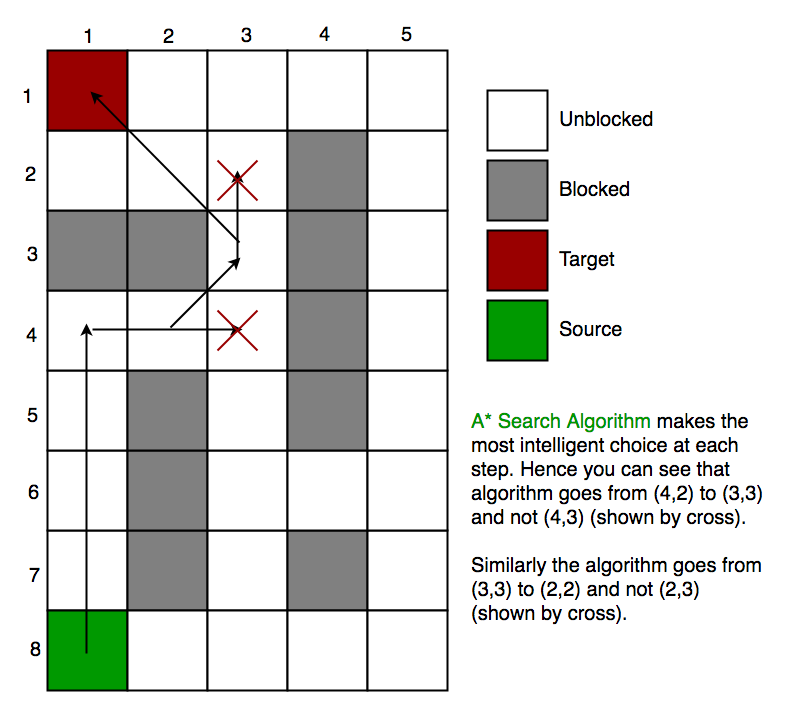
\includegraphics[width=\linewidth]{img/a_-search-algorithm.png}
        \caption{Astar path}
        \label{fig:astar_path}
        	
    \end{subfigure}
	\hspace{0.02\textwidth}
	\begin{subfigure}[b]{0.3\linewidth}
		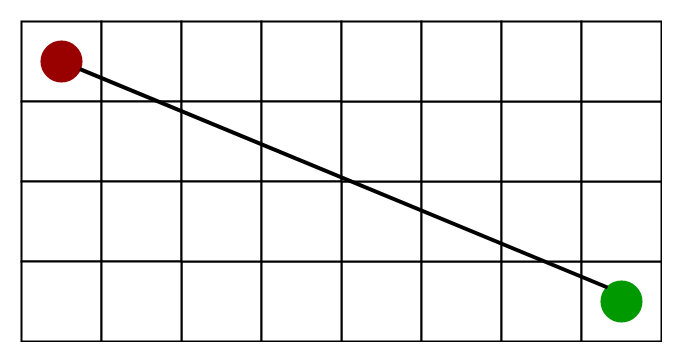
\includegraphics[width=\linewidth]{img/a_-search-algorithm-euclidian_distance.png}
		\caption{Euclidean Distance Heuristics}
        \label{fig:EuclideanDistanceHeuristics}
	\end{subfigure}
 	\caption{A* algorithm \cite{Pic:astar}}
	\label{fig:astar}
    \vspace{-15pt}
\end{figure}

Algorithm steps: \cite{app9061057} \newline
\textbf{step 1:} Insert the starting node into a priority queue.
\newline
\textbf{step 2:} Choose the node with the lowest F value from the current queue and assign it as the current node.
\newline
\textbf{step 3:} Mark the current node as visited and process its neighbor nodes.
\newline
\textbf{step 4:} If the neighbor node has not been visited yet, add it to the queue, set the current node as its parent, and record its F, H, and G values.
If the neighbor node has already been visited, compare the G values to determine if the current node has a shorter path. See figure \ref{fig:astar_path}.
If the current node has a smaller G value, update the parent node and the G and H values of that node.
\newline
\textbf{step 5:} Repeat steps 2 through 4 until the target node is marked or the priority queue is empty.
\newline
\textbf{step 6:} Once the path is discovered, follow the parent node from the endpoint to the start node.





\newpage
\subsection{La-MCTS}
The basic idea of a \ac{La-MCTS} is to recursively partition the search space, where each region represents a node in a Monte Carlo tree.\cite{La-MCTS}
As shown in Figure \ref{fig:laMCTS_sampling_splitting}, this is done by taking some samples from the search space and splitting them into a high reward region and a low reward region using K-means (k=2).
A \ac{SVM} then learns this boundary, and the two sections can be represented as nodes in a Monte Carlo tree.
In our example, the high reward section is represented by the left node and the low reward section is represented by the right node.


\begin{figure}[H]
	\centering
	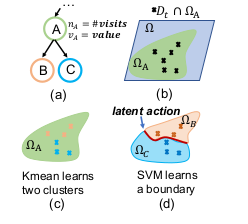
\includegraphics[width = {0.35\textwidth}]{img/lamcts_1.png}
	\caption{\ac{La-MCTS} sampling and splitting \cite[p.3]{La-MCTS}}
	\label{fig:laMCTS_sampling_splitting}
    \vspace{-20pt}
\end{figure}
As shown in Figure \ref{fig:laMCTS_workflow}, this process is now repeated by selecting a node until a leaf node is reached, sampling along the corresponding section, and splitting it again.
The result is a tree structure where the leftmost node represents the section with the highest reward. 

\begin{figure}[H]
	\centering
	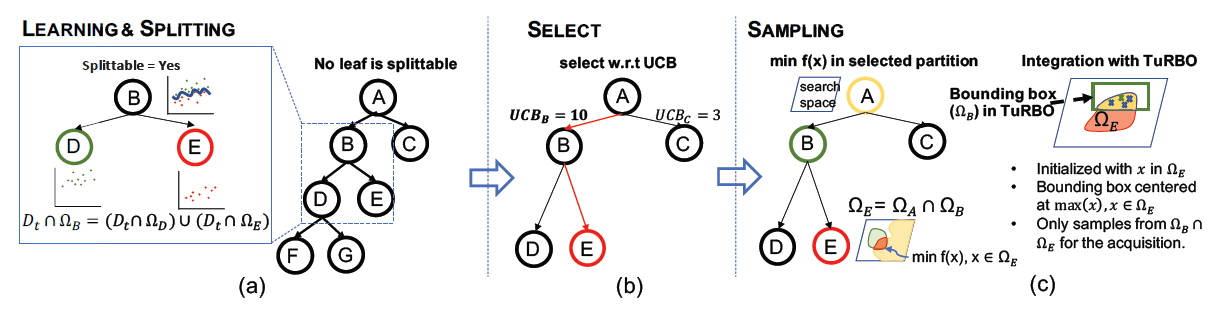
\includegraphics[width = {\textwidth}]{img/lamcts_workflow.png}
	\caption{Steps of \ac{La-MCTS} \cite[p.4]{La-MCTS}}
	\label{fig:laMCTS_workflow}
    \vspace{-20pt}
\end{figure}

\subsection{LaP3}
%https://www.youtube.com/watch?v=-4Lzk_s_Dzw
\ac{LaP3} functions similarly to \ac{La-MCTS}. The main difference is that the entire tree is updated after each sampling step, rather than a single leaf. Other differences include the method used to determine the goodness of a node (\ac{LaP3} uses the maximum, while \ac{La-MCTS} uses the mean) and the sampling method (\ac{LaP3} uses \ac{CMA-ES}, while \ac{La-MCTS} uses \ac{BO}). \cite{NEURIPS2021_03a3655f} \cite{La-MCTS}
\begin{comment}
LaMCTS samples aus einzelnen regionen, lap3 sampled einmal am anfang
ganze tree wird nicht geupdatet
\end{comment}

\section{Methodology}
We ran \ac{LaP3}, \ac{La-MCTS}, and an A* on two different environments, with both environments containing local optima.
For each environment, the experiment was run on a 12x12, a 24x24, and a 36x36 grid.
Since the goal is to find a sampling efficient trajectory, the number of samples was used as a metric in relation to the reward.
The reward was calculated by the inverse of the Euclidean distance to the target. It can be described by the following formula.

\begin{equation}
\left\{
\begin{array}{lll}
 r(\vec{x})=\frac{10}{\sqrt{\Delta x_1 ^2+\Delta x_2 ^2}}\quad&, \Delta x_1 + \Delta x_2 \neq 0\\
r(\vec{x})=15 &,\quad \Delta x_1 + \Delta x_2 =0\\
\end{array}
\right.
\end{equation}
%100 laufen lassen erst in evaluation

\begin{figure}[H]
	\centering
	\begin{subfigure}[b]{0.3\linewidth}
		\includegraphics[width=\linewidth]{img/Maze_s3.png}
        \caption{Maze S3}	
    \end{subfigure}
	\hspace{0.02\textwidth}
	\begin{subfigure}[b]{0.3\linewidth}
		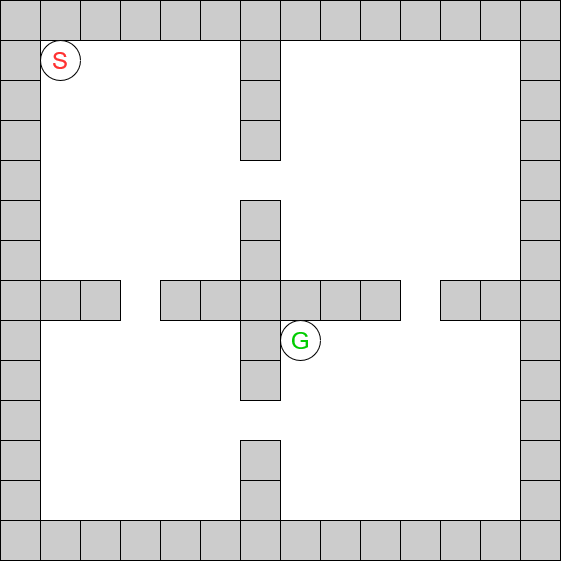
\includegraphics[width=\linewidth]{img/Four_Rooms.png}
		\caption{Four Rooms}
	\end{subfigure}
 	\caption{different environments}
	\label{fig:differentenvironments}
\end{figure}

\subsection{Search Efficiency}
The goal in path planning is to find the most rewarding trajectory in the search space.
Since the optimum can eventually be found by random sampling, if the number of samples is high enough, an efficient algorithm is preferred.
Therefore, the search efficiency of an algorithm can therefore be described by the number of samples and the achieved reward.
Since this metric is widely used in comparing different search algorithms, \cite{La-MCTS}, \cite{LaNAS}, \cite{VOOT}, we also used it for comparison.
\newpage
\section{Evaluation}

%1. LaP3 Algorithmus wurde entwickelt, der die Pfade schneller berechnet
%2. LAP3 performt besser als der MCTS und A*
%3. Anhand gleicher Anzahl an samples ist der reward beim LAP3 immer besser
%4. verschiedene Metriken wurden verwenden space complexity, world environment
%5. Was sind unsere Ergebnisse, Performt LAP3 tatsächlich immer besser?
%6. Was kann in Zukunft noch nageschaut werden?

The algorithms were ran in different environments, to see if \ac{LaP3} performs better with respect to sample efficiency.
%With the evaluation criterion sample efficiency and the different environment, the search algorithms are examined to see if the \ac{LaP3} performs better from several points of view.
Figure \ref{fig:SampleRewardMazeDifferentSpaceComplexity} shows the number of samples drawn and the associated reward in different environments with different complexities.
The environment is maze s3 with complexity sizes 12x12, 24x24 and 36x36
A* always yields the same results, but \ac{La-MCTS} and \ac{LaP3} deliver different results for a hundred runs. 
Therefore, the mean and the lower and upper bounds of the 95 confidence interval are shown in the graphs.
It can be seen that \ac{LaP3} receives a larger reward than \ac{La-MCTS} and A* with the same number of samples.
Although \ac{LaP3} has a high variance, the reward increases steadily as the number of samples increases.
However, the \ac{LaP3} algorithm has a very large variance in the results provided.
For \ac{La-MCTS}, an increase in variance does not occur until a sample size of 42 in a 12x12 environment and a sample size of 55 in a 24x24 and 36x36 environment.
The reward of A* varies continuously, but the reward does not increase as the number of samples increases.

\begin{figure}[H]
	\centering
	\begin{subfigure}[b]{0.3\linewidth}
		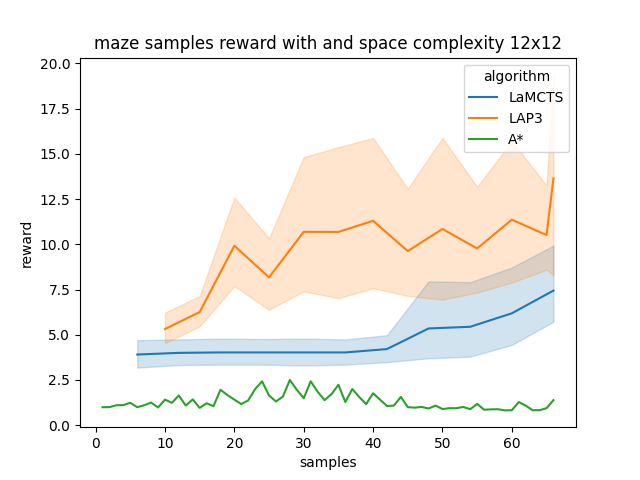
\includegraphics[width=\linewidth]{img/maze_samples__reward_b_8_LAP3_MCTS_AStar_interrupted_12.png}
        \caption{space complexity 12x12}	
    \end{subfigure}
	%\hspace{0.02\textwidth}
	\begin{subfigure}[b]{0.3\linewidth}
		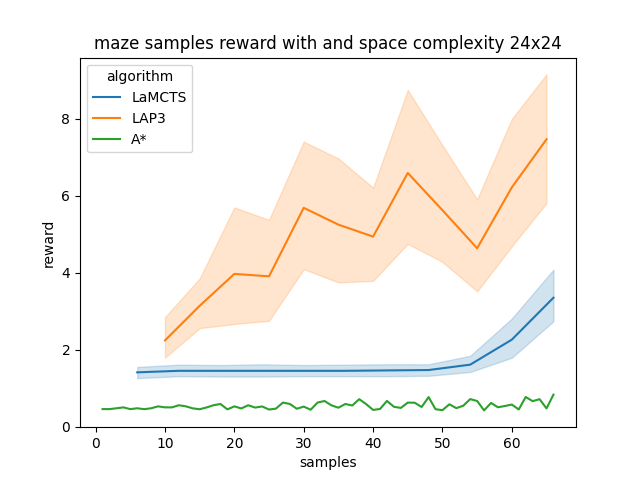
\includegraphics[width=\linewidth]{img/maze_samples__reward_b_8_LAP3_MCTS_AStar_interrupted_24.png}
		\caption{space complexity 24x24}
	\end{subfigure}
	%\hspace{0.02\textwidth}
	\begin{subfigure}[b]{0.3\linewidth}
		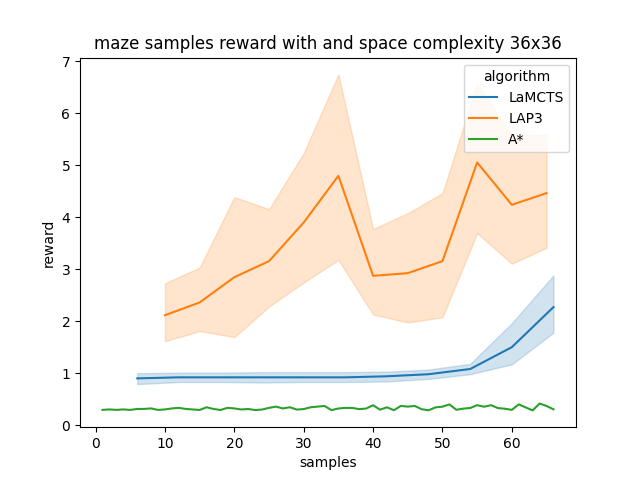
\includegraphics[width=\linewidth]{img/maze_samples__reward_b_8_LAP3_MCTS_AStar_interrupted_36.png}
        \caption{space complexity 36x36}
	\end{subfigure}
	\caption{number of samples and reward in Maze s3 environment with different space complexity}
	\label{fig:SampleRewardMazeDifferentSpaceComplexity}
\end{figure}

Figure \ref{fig:SampleRewardFourRoomsDifferentSpaceComplexity} shows the number of samples drawn and the associated reward in the four rooms environment with complexity sizes of 12x12, 24x24, and 36x36.
As in the maze s3 environment, A* produces a low reward with a low number of samples.
Only in the 12x12 environment with a sample number of 40 does the reward increase and achieve a similar reward as the \ac{La-MCTS}.
At greater space complexity, the reward remains consistently low.
The \ac{La-MCTS} corresponds to a growing exponential function with constant mean.
The \ac{LaP3}, on the other hand, has a strong growth in rewards at the beginning.
However, as the sample number, however, the growth decreases.
However, \ac{LaP3} has a higher reward than \ac{La-MCTS} and A* for each number of samples.

\begin{figure}[H]
	\centering
	\begin{subfigure}[b]{0.3\linewidth}
		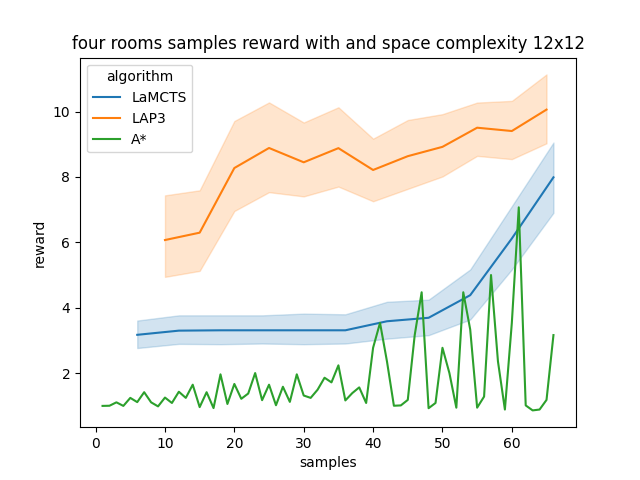
\includegraphics[width=\linewidth]{img/four_rooms_samples__reward_b_8_LAP3_MCTS_AStar_interrupted_12.png}
        \caption{space complexity 12x12}	
    \end{subfigure}
	\hspace{0.02\textwidth}
	\begin{subfigure}[b]{0.3\linewidth}
		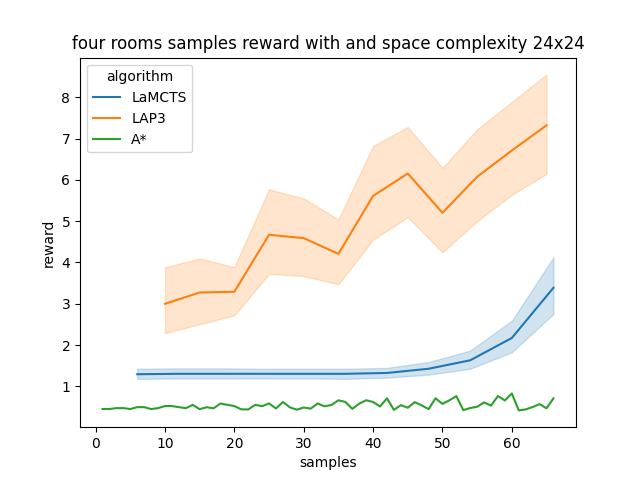
\includegraphics[width=\linewidth]{img/four_rooms_samples__reward_b_8_LAP3_MCTS_AStar_interrupted_24.png}
		\caption{space complexity 24x24}
	\end{subfigure}
	\hspace{0.02\textwidth}
	\begin{subfigure}[b]{0.3\linewidth}
		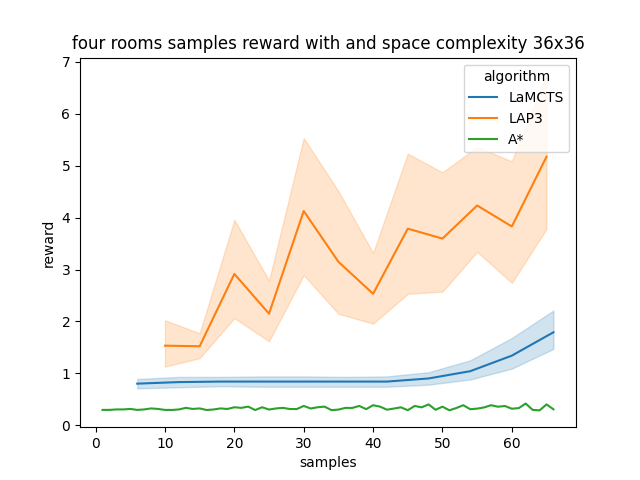
\includegraphics[width=\linewidth]{img/four_rooms_samples__reward_b_8_LAP3_MCTS_AStar_interrupted_36.png}
        \caption{space complexity 36x36}
	\end{subfigure}
	\caption{number of samples and reward in four rooms environment with different space complexity}
	\label{fig:SampleRewardFourRoomsDifferentSpaceComplexity}
\end{figure}

What we have seen in the previous comparisons in the maze s3 and four rooms environment, the \ac{LaP3} always has a better reward per drawn samples.
However, the results of the algorithms depend on the environment in which they are executed.
As can be seen in Figure \ref{fig:SampleRewardMazeDifferentSpaceComplexityAlgo}, it can also be seen that the \ac{LaP3} performs most robustly when the space complexity is increased.
The reward of the A* is small with increasing complexity and almost does not increase.
On the other hand, the \ac{La-MCTS} shows similar behavior of rewards at different spatial complexities.

\begin{figure}[H]
	\centering
	\begin{subfigure}[b]{0.3\linewidth}
		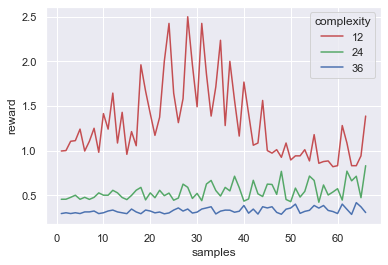
\includegraphics[width=\linewidth]{img/maze_sample_reward_astar.png}
        \caption{A*}	
    \end{subfigure}
	\hspace{0.02\textwidth}
	\begin{subfigure}[b]{0.3\linewidth}
		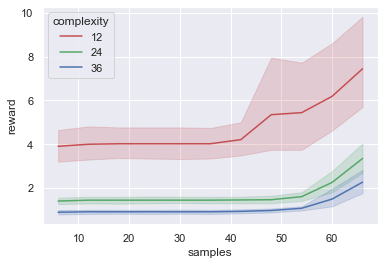
\includegraphics[width=\linewidth]{img/maze_sample_reward_lamcts.png}
		\caption{LaMCTS}
	\end{subfigure}
	\hspace{0.02\textwidth}
	\begin{subfigure}[b]{0.3\linewidth}
		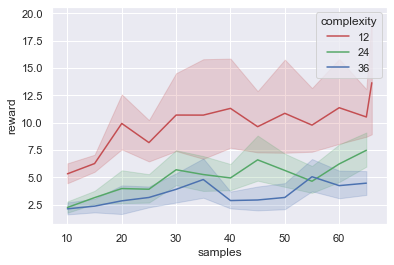
\includegraphics[width=\linewidth]{img/maze_sample_reward_lap3.png}
        \caption{LaP3}
	\end{subfigure}
	\caption{number of samples and reward in maze s3 environment}
	\label{fig:SampleRewardMazeDifferentSpaceComplexityAlgo}
\end{figure}

\begin{comment}
What is striking in both environments is that \ac{La-MCTS} has a constant reward function between 10  and 40 samples. 
After 40 samples the reward seems to exponentially increase.


    
The \ac{LaP3} exhibits significant variation in its reward data, although the specific mean values provided by the \ac{LaP3} are displayed in Figure \ref{tab:mean_std_diff_sizes}. 
As we can see in Figure \ref{fig:maze_complexity_reward_lap3_lamcts_astar}, the complexity of the environment increases, the reward diminishes rapidly.

\begin{figure}[H]
	\centering
	\begin{subfigure}[b]{0.55\linewidth}
    	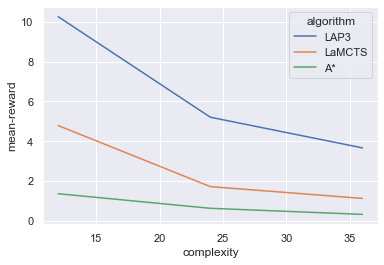
\includegraphics[width = {\textwidth}]{img/maze_complexity_reward_lap3_lamcts_astar.png}
    	\caption{maze s3 space complexity and mean reward $\overline{x}$}
    	\label{fig:maze_complexity_reward_lap3_lamcts_astar}	
    \end{subfigure}
	%\hspace{0.02\textwidth}
    \begin{subfigure}[b]{0.4\linewidth}
        \begin{tabular}{|c|c|c|c|c|}
        \hline
        & {12x12} & {24x24} & {36x36} \\ \hline
        Samples & $\overline{x}$ & $\overline{x}$ &  $\overline{x}$ \\ \hline
        20 &  9.9208     & 3.9697  & 2.8462 \\ \hline
        25 &  8.1711     & 3.9062  & 3.1538 \\ \hline
        30 &  7.4318     & 5.6875  & 3.8974 \\ \hline
        35 & 10.6842     & 5.2500  & 4.7949 \\ \hline
        40 & 11.3000     & 4.9394  & 2.8718 \\ \hline
        45 &  9.6250     & 6.5938  & 2.9231 \\ \hline
        50 & 10.8485     & 5.6250  & 3.1538 \\ \hline
        55 &  9.7692     & 4.6364  & 5.0513 \\ \hline
        60 & 11.3611     & 4.6364  & 4.2368 \\ \hline \hline
           & 10.2632     & 5.2030  & 3.6588 \\ \hline
        \end{tabular}
        \caption{mean and 95\% confidence interval of \ac{LaP3}}
        \label{tab:mean_std_diff_sizes}
    \end{subfigure}
    \caption{first 60 samples drawn in maze s3 environment with different complexity}
    %\label{fig:mean_complexity_reward}
\end{figure}
\end{comment}
%\todo[inline]{Aussage beantwortet, \ac{LaP3} performt immer besser}
%\todo[inline]{Schaubild 7 beschreiben}
%\todo[inline]{\ac{LaP3} beschreiben, dass man in ein locales minumu leicht reinkommt}
\newpage
\section{Conclusions and Further Discussion}
The data clearly show that \ac{LaP3} outperforms other path planning algorithms in different environments, as claimed by the authors.
\ac{LaP3} has a greater ability to deal with uncertainty and stochastic models.
A* requires a deterministic heuristic function and \ac{LaP3} uses a probabilistic procedure to achieve the goal.
This can be to the advantage of \ac{LaP3} when the algorithm is run in dynamic environments and in environments with incomplete information.
\ac{LaP3} may be able to detect that a certain path leads to collisions or obstacles.
However, we did not examine the single improvements of \ac{LaP3} over \ac{La-MCTS}, such as the whole tree update, the different sampling methods, and the different computation of node quality and their partial impact on search efficiency.
In addition, search efficiency could be measured not in absolute terms (number of samples), but based on the size of the search space they explore. 
This would facilitate the comparison of different space complexities (12x12, 24x24, etc.).
It would also be interesting to know if \ac{LaP3} would still outperform the other algorithms by the same amount if sampling the entire search space were not possible.

%The aim is to prove that the \ac{LaP3} algorithm has a better result than its forerunners \ac{La-MCTS} and A* under different conditions.



%\todo[inline]{functions evals?, Manuel, haben nix gemacht wird aber im paper benutzt}
%\todo[inline]{sample drawing in sequential action space (horiyon tto draw %samples from, not whole search space), Manuel}
%\todo[inline]{Wie performt LaP3 in größeren Umgebungen}

%\clearpage


\section*{Acronyms} 
\addcontentsline{toc}{section}{Acronyms}

\begin{acronym}[....]
    \acro{LaP3}{Latent Space Partitions for Path Planning}
    %\acro{MCTS}{Monte Carlo Tree Search}
    \acro{La-MCTS}{Latent Action Monte Carlo Tree Search}
    %\acro{LaNas}{Latent Space Neural Architecture Search}
    \acro{CMA-ES}{Covariance matrix adaptation evolution strategy}
    \acro{BO}{Bayesian Optimization}
    \acro{VOOT}{Voronoi Optimistic Optimization Tree}
    \acro{SVM}{support vector machine}
\end{acronym}

\bibliographystyle{alpha}
\bibliography{literature}
\end{document}
